% !TEX root = /home/eb/.vscode/qftrules.prepaworkshop/tmp/Exercice.tex
%%%%%%%%%%%%%%%%%%%%%%%%%%%%%%%%%%%
\begin{exo}[1][devoir]{Interféromètre de Fabry-Perot}
  Un interféromètre de Fabry-Perot est constitué d'une lame d'air à faces parallèles d'épaisseur $e$ comprise entre deux lames de verre d'épaisseur négligeable. Ces lames ont un coefficient de transmission en amplitude $t$ et un coefficient de réflexion en amplitude $r$.
  On éclaire la lame avec une source étendue monochromatique de longueur d'onde $\lambda=\SI{422,7}{nm}$. Un rayon incident donne naissance à différents rayons dont on doit tenir compte si le coefficient de réflexion est élevé.
  \begin{center}
  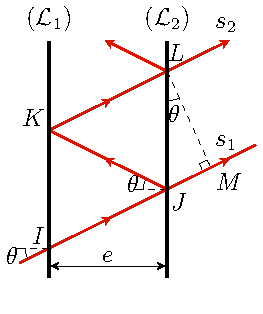
\includegraphics[scale=1]{Diff_marche.pdf}
  \end{center}
  \begin{questions}
    \item Quelle relation existe-t-il entre $r$ et $t$ si l'on néglige l'absorption lumineuse. On rappelle que les coefficients de réflexion et transmission en énergie sont données par $r^2$ et $t^2$. 
    \solution{
    Par conservation de l'énergie, on a 
    $$\boxed{
      r^2 + t^2 = 1.
    }$$
    }
    \item En s'aidant du théorème de Malus et de constructions géométriques, déterminer le déphasage constant $\varphi$ entre deux rayons émergents successifs en fonction de $e, \lambda$ et $\theta$.
    \solution{
    On a $\delta = 2e \cos \theta$ (la démo sera faite pour le Michelson en lame d'air) et donc 
    $$\boxed{
      \varphi = \frac{2\pi}{\lambda} \delta = \frac{4\pi e}{\lambda} \cos \theta.
    }$$
     Le calcul de la différence de marche se fait comme dans le cours sur la division d'amplitude.
    }
    \item On appelle $\underline{s}_m$ l'amplitude complexe de l'onde associée au $m$-ième rayon. Quelle relation a-t-on entre $\underline{s}_{m}$ et $\underline{s}_{m-1}$ ? Comment s'exprime $\underline{s}_m$ en fonction de $\underline{s}_1$ ? En déduire l'expression de l'amplitude résultante $\underline{s}$ et montrer que l'intensité lumineuse $I$ à pour expression 
    $$
  I=\frac{I_{\rm max}}{1+m \sin ^2(\frac{\varphi}{2})},
  $$
  où  l'on supposera $r$ réel et où $m$ est à déterminer.
  \solution{
    On a $\underline{s}_{m+1} = r^2 \underline{s}_m e^{i\varphi}$. En effet, chaque aller-retour entre les lames de verre s'accompagnent de deux réflexions. 
    On utilise la méthode de sommation du cours pour les interférences à $N$ ondes. On a 
    $$\underline{s} = \sum_{k=1}^{\infty} \underline{s}_k = \underline{s}_1 \sum_{k=0}^{\infty} r^{2k} e^{i k \varphi} = \underline{s}_0\frac{1}{1-r^2e^{i\varphi}}.$$
    l’intensité vaut donc 
    $$
  I = \frac{1}{2} \underline{s} \underline{s}^\star = \frac{I_0}{(1-r^2\cos\varphi)^2 + r^4 \sin^2(\varphi) } = \frac{I_0}{1 - 2r^2\cos\varphi + r^4} = \frac{I_{\rm max}}{(1-r^2)^2 + 4r^2 \sin^2(\frac{\varphi}{2})},
    $$
    en utilisant la formule $\cos(2a) = 1-2\sin^2(a)$. On a donc
    $$
    I_{\rm max} = \frac{I_0}{(1-r^2)^2}.
    $$ 
    $$\boxed{
      m = \frac{4r^2}{(1-r^2)^2}.
    }$$}
  \item Représenter l'intensité $I$ en fonction de $\varphi$ pour différentes valeurs de $r$. On désire des interférences très contrastées. Comment faut-il choisir $r$ ?
  \solution{
    On a représenté ci-dessous le graphe de la fonction $I(\varphi)$ (fonction d'Airy) pour plusieurs valeurs de $R=r^2$ (coefficient de réflexion en intensité).
    \begin{center}
      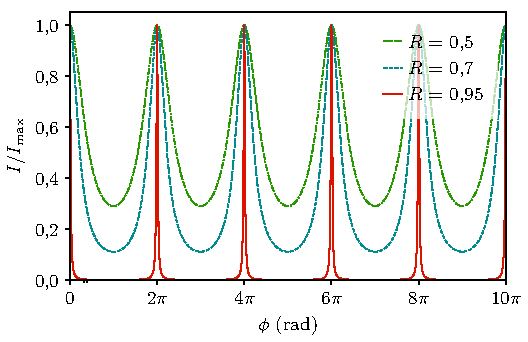
\includegraphics[width=0.7\columnwidth]{Fonction_airy_new.pdf}
    \end{center}
  Le contraste vaut $\mathcal{C}\simeq 1$ car l'intensité  minimale est quasi nulle pour $m$ grand. Mais les franges brillantes sont d'autant mieux séparées les unes des autres que $r$ est grand.  On le verra ci-après en calculant la finesse.
  }
  \end{questions}
  \end{exo}
  %%%%%%%%%%%%%%%%%%%%%%%%%%%%%%%%%%%
  